% Auto-generated editable source. Edit freely in VS Code.
% This is a parallel source; the live site is the .html file at pages/proj-action-identifiability.html.
\documentclass[11pt]{article}
\usepackage[margin=1in]{geometry}
\usepackage{graphicx}
\usepackage{hyperref}
\usepackage{enumitem}
\usepackage{xcolor}
\definecolor{aidred}{HTML}{A8324A}
\definecolor{aidpink}{HTML}{CF4D87}
\hypersetup{colorlinks=true,linkcolor=aidpink,urlcolor=aidpink,citecolor=aidpink}
\newcommand{\finding}[2]{\par\medskip\noindent{\color{aidred}\textbf{Finding #1.}}~#2\par\medskip}
\newcommand{\stat}[2]{\par\medskip\begin{center}{\LARGE\textbf{\textcolor{aidred}{#1}}}\\[2pt]{\small #2}\end{center}\par\medskip}

\title{Action Identifiability in Protein-Design Agents}
\author{Saanvi S. Subramanian \\ \small California Institute of Technology}
\date{\small poster, AgenticLS @ NeurIPS 2026 \quad\textbullet\quad MoML 2026 (MIT) \quad\textbullet\quad sole author}
\begin{document}
\maketitle

\begin{abstract}
\noindent A protein-design agent proposes a biological action, enacts it as a displacement in a protein model's representation, and scores the result in that same representation. This works only if the representation keeps distinct actions apart. I test whether it does, with ESM-2 and the 78 COSMIC somatic mutational signatures as the action space. Across all 3{,}003 signature pairs, biologically distinct processes often reach the same ESM-2 destination, and the separation that remains tracks broad substitution composition rather than the trinucleotide context that defines a signature. A probe can still decode which process produced a displacement at 66\% against 20\% chance, but its errors merge processes the catalogue holds apart, and the design objective shares the representation it is scored in. On this evidence the agent should return the compatible set or abstain, not name one process.
\end{abstract}

\section*{The setup}
The testbed is a hypothesise-simulate-validate loop for mutational-driver discovery. The agent proposes a mutational process, enacts its mean hidden-state displacement by activation steering, and compares the enacted direction against the displacement the measured mutation caused. A mutational signature is a process's characteristic pattern of base substitutions in its local three-letter context, and COSMIC catalogues 78 of them. The action space is these 78 processes, and the question is whether the representation the agent acts through can tell them apart. If two processes reach the same destination, no amount of calibration recovers the difference.

\section*{Distinct processes reach the same place}
Three biologically distinct processes, SBS1 (clock-like), SBS7a (UV) and SBS2 (APOBEC), land at pairwise cosine distance at or below 0.011, while SBS17a sits out at 0.04 to 0.08. The collapse is not just the catalogue's own structure. SBS2 and SBS7a do have similar spectra, at cosine 0.71, but SBS2 and SBS1 are near-orthogonal in COSMIC at cosine 0.02 and still merge in ESM-2. The representation is collapsing a distinction the catalogue makes.

\paragraph{What the composition control shows.} Scrambling trinucleotide context while preserving each substitution type's marginal probability moves the destination by $0.0081 \pm 0.0016$, against a seed-to-seed floor of $0.0014 \pm 0.0005$. Context does register, $5.8\times$ above the sampling floor, but the effect is 3.6 to $7.3\times$ smaller than the separation between signatures with different substitution composition. The three collapsed processes are all C$>$T dominated and SBS17a is T$>$C dominated, which is the composition axis, not the biology.

\finding{1}{Across all 3{,}003 pairs of the 78 COSMIC signatures, biologically distinct mutational processes often reach similar ESM-2 destinations, and the separation that does exist tracks broad substitution composition rather than the trinucleotide context that defines the signatures. An agent in this representation should return the compatible set or abstain, not name one process.}

\finding{2}{The measurement procedure did much of the work. Stop-at-first-stop translation turns 524 of 2{,}028 simulated mutants, 25.8\%, into one-residue placeholders, and per-signature placeholder count alone explains $R^2 = 0.683$ of pairwise destination distance at 8M and 0.870 at 650M. A length control removes the artifact, but the binary collapse rate is then strongly scale-dependent, 23.8\% of pairs at or below the 0.011 threshold at 8M against 72.5\% at 650M. I report both and do not pick one as a catalogue-wide rate.}

\begin{figure}[h]
\centering
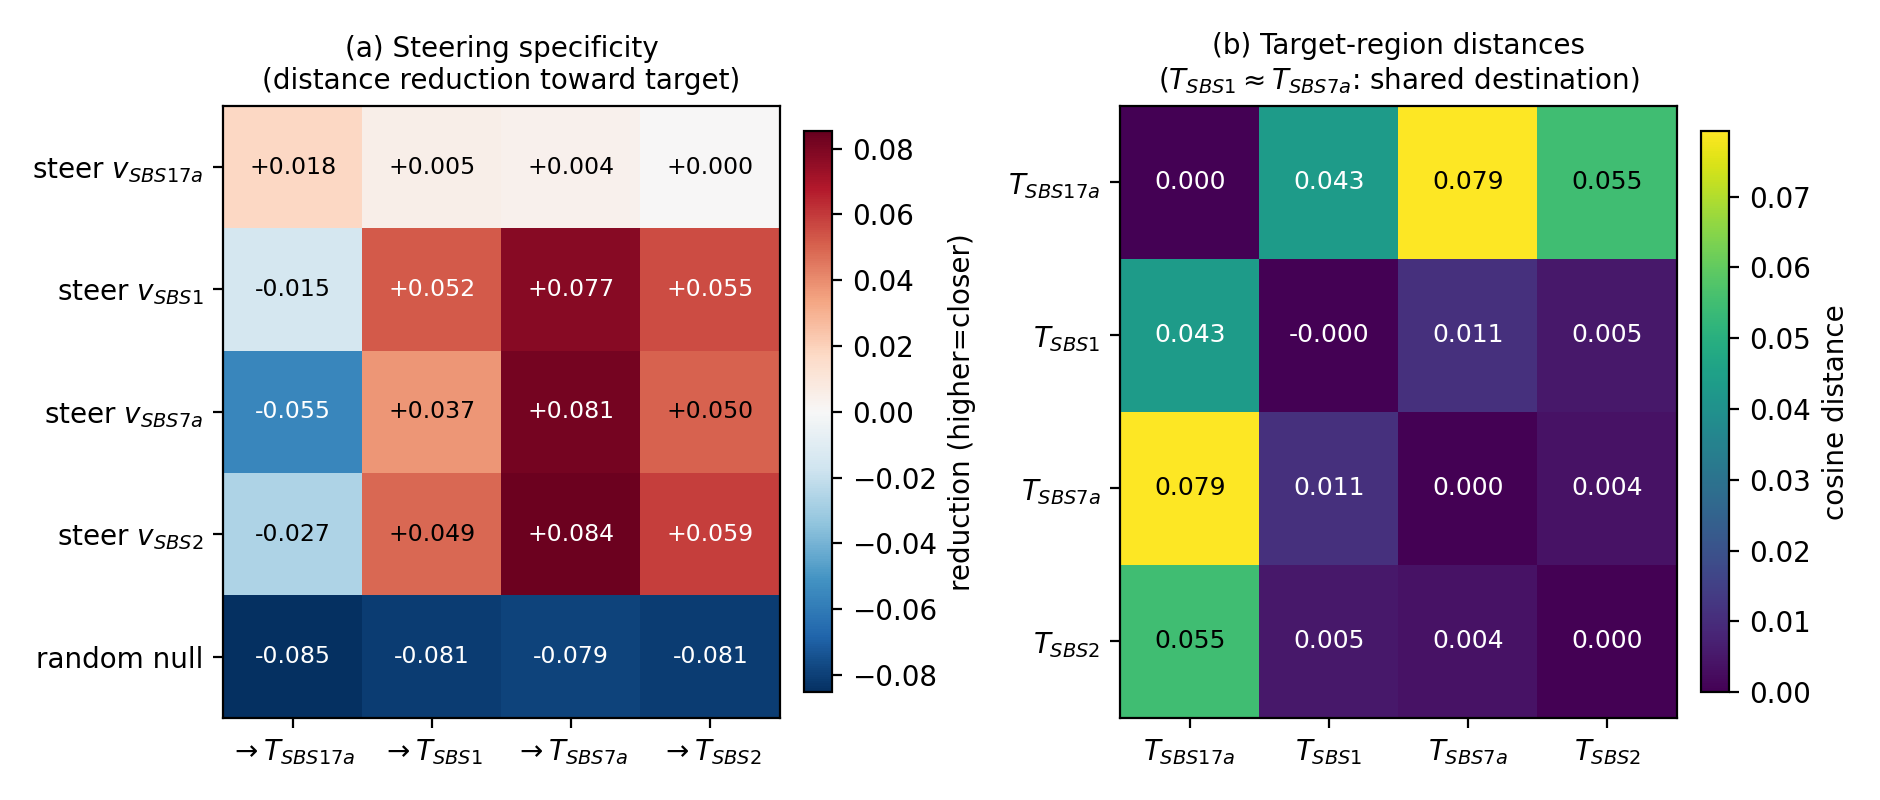
\includegraphics[width=\textwidth]{../../assets/images/projects/agentevals/identifiability-signatures.png}
\caption*{\textcolor{aidred}{\textbf{Figure 1. Action-space identifiability in ESM-2 8M.}} Left, the steering cross-matrix: enacting each mutational process moves held-out proteins toward its own outcome region, with SBS1, SBS7a and SBS2 overlapping while SBS17a sits farther out. Right, the same pattern in pairwise destination distance. The 0.011 line is inherited from the original four-signature experiment, so read it as a reference rather than a verdict.}
\end{figure}

\section*{What the representation can and cannot decode}
The representation is not empty. A probe that reads an ESM-2 displacement and names which of five processes produced it reaches 66\% five-way accuracy against 20\% chance, and 89\% on SBS17a. The structure of the errors is the finding. The confusions are not random, and SBS1 is confused with SBS2 even though their COSMIC spectra are near-orthogonal at cosine 0.02. The representation decodes a real signal and still merges processes the catalogue separates.

\begin{figure}[h]
\centering
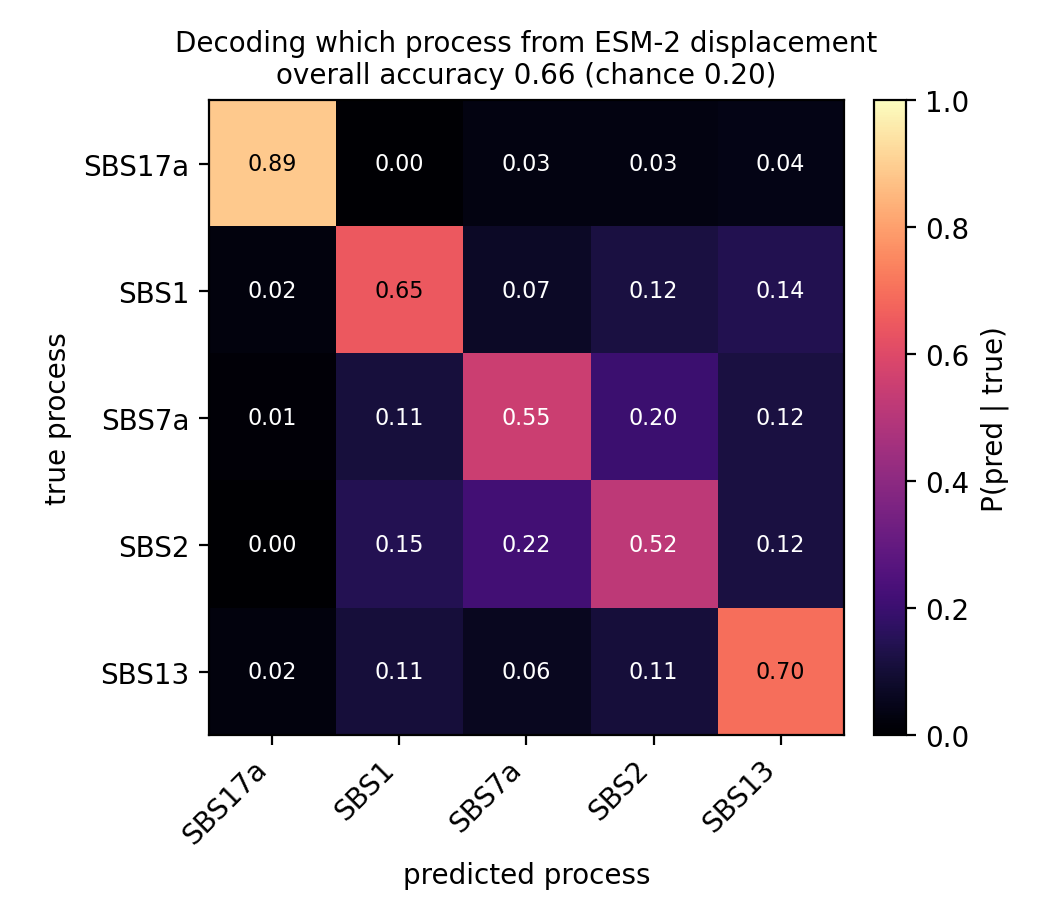
\includegraphics[width=\textwidth]{../../assets/images/projects/agentevals/identifiability-decoding.png}
\caption*{\textcolor{aidred}{\textbf{Figure 2. What the representation can and cannot decode.}} A probe decoding which of five mutational processes produced a displacement reaches 66\% five-way accuracy against 20\% chance, and 89\% on SBS17a, so the representation carries signal. The off-diagonal is the point: SBS1 is confused with SBS2 despite near-orthogonal COSMIC spectra, so the errors follow composition rather than the catalogue.}
\end{figure}

\finding{3}{The embedding-proximity objective is exploitable, and the validation check shares its representation. An agent making unconstrained single-residue edits drives cosine distance to the PF17041 centroid from 0.26 to 0.009 over 200 edits, landing 5.0 standard deviations below the natural-protein reference mean of $0.194 \pm 0.037$ across 25 measured proteins, while ESM-2 naturalness falls from $-0.41$ to $-0.50$, 2.2 sd below the natural band. The removed plausibility signal does detect the departure, but because both the objective and the causal self-validation score live in ESM-2, validation in the same representation is not independent evidence against this failure.}

\paragraph{Why the 0.011 threshold needs hedging.} It was defined from the SBS1 to SBS7a distance in the original four-signature 8M uncontrolled experiment, and it does not carry the same meaning elsewhere. It contains the SBS1, SBS7a and SBS2 reference cluster in two of the four model-by-readout conditions and splits it in the other two. Picking the condition where it behaves after seeing the result would overstate collapse, so the catalogue-wide conclusion rests on continuous distances and within-process spread instead.

\section*{Limitations}
The steering and decoding experiments cover a subset of signatures while the destination analysis covers all 78, so catalogue-wide overlap is established and per-signature steering specificity is not. ESM-2 8M and 650M share training data and tokenisation, so the scale comparison is not an independent-model replication. The unconstrained optimisation result shows this objective can be exploited under single-residue search, not that every constrained design objective fails the same way. A matched-compute control also erases the apparent agency gain: at 100 scorer calls, fixed and random search reach final centroid distances of 0.1586 and 0.1585 against 0.1625 for the adaptive policy, so the adaptive policy has no measured advantage on those 20 protein-goal tasks. That control does not touch the identifiability result, but it is why this poster reports position only.

\end{document}
